\section{Parallele Rechnermodelle}
Eine paralleles Modell zeichnet sich dadurch aus, dass mehrere Instruktionen gleichzeitig von Prozessoren ausgeführt werden.
Eine parallele Maschine arbeitet \emph{synchron}, wenn in jedem Schritt alle Prozessoren gleichzeitig eine Instruktion ausführen.
Die Instruktionen müssen nicht unbedingt identisch sein.
Andernfalls arbeitet die Maschine \emph{asynchron}.
Führen alle Prozessoren die gleichartige Instruktionen zur gleichen Zeit aus, wird dies \emph{Single Instruction Multiple Data (SIMD)} genannt; unterscheiden sich die Programme, so lautet die Bezeichnung \emph{Multiple Instructions Multiple Data (MIMD)}.

\subsection{Circuit}
Ein Circuit ist ein Repräsentation als gerichteter azyklischer Graph (engl. directed acyclic graph, DAG) mit benannten Knoten.
Knoten ohne eingehende Kanten, die Blätter, stellen die Eingaben dar, Knoten ohne ausgehende Kanten, die Wurzeln, die Ausgaben.
Die Knoten mit eingehenden Kanten sind mit den Operationen beschriftet, die jeweils in einer Zeiteinheit über maximal zwei Operanden, den eingehenden Kanten, ausgeführt werden.
Die Zeitkomplexität eines Circuit ist die Tiefe des DAG.

Ein Circuit kann aus einem Straight Line Program abgeleitet werden, indem jede Variable, der mehrfach ein Wert zugewiesen wird, durch entsprechend viele neue Variablen ersetzt wird.
Die Knoten des Circuits entsprechen dann den verschiedenen Variablen aus dem SLP.
Die Blätter entsprechen den Eingabevariablen.
Die restlichen Knoten sind mit den Operationen der entsprechenden Variablenzuweisung beschriftet und haben eintreffende Kanten ausgehend von den Abhängigkeiten der Zuweisung.
Ist das SPL boolesch, so spricht man von einem \emph{boolean circuit}.
\cite[S.7]{jaja}\cite[S.11f.]{reif}

\paragraph{Beispiel}
Zwei verschiedene Ansätze, die Summe aus acht Zahlen zu bilden, sind in
Abbildung \ref{circuit} dargestellt.
Circuit $A$ berechnet alle sieben Präfixsummen, addiert alle acht Zahlen
nacheinander.
$A$ besitzt eine Zeitkomplexität von $time = 7$.
$B$ hingegen berechnet Teilsummen parallel.
Der Baum ist flacher, der Algorithmus hat eine Zeitkomplexität von $time = 3$.

\begin{figure}
    \centering
    % two circuits computing the sum of eight numbers
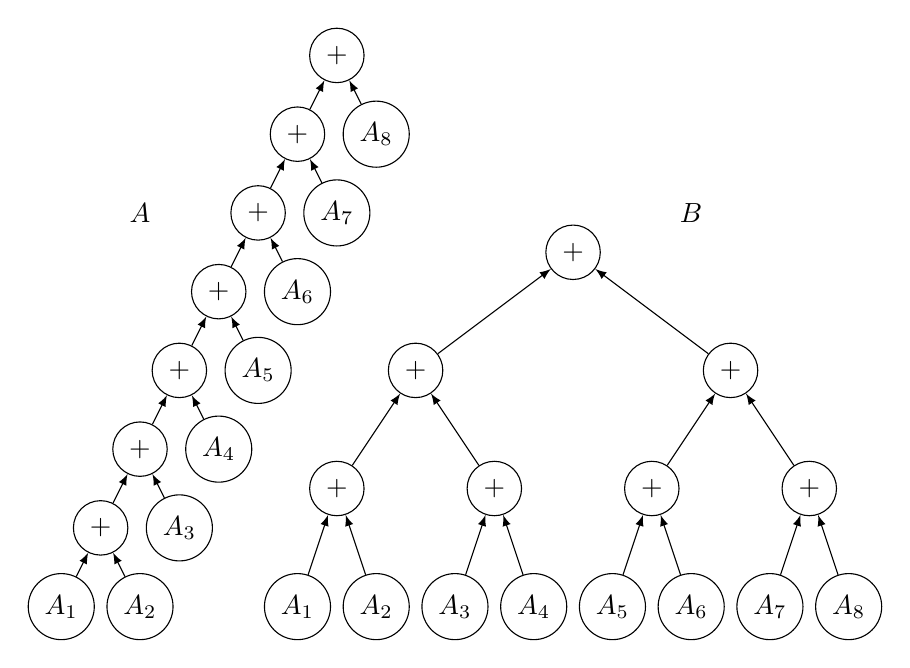
\begin{tikzpicture}
    [
        vertex/.style={circle, draw, scale=1, minimum size=3ex,},
        edge/.style={-latex,},
    ]

    % parallel dag
    \node (a1) at (0,0)     [vertex] {$A_1$};
    \node (a2) at (1,0)     [vertex] {$A_2$};
    \node (a3) at (2,0)     [vertex] {$A_3$};
    \node (a4) at (3,0)     [vertex] {$A_4$};
    \node (a5) at (4,0)     [vertex] {$A_5$};
    \node (a6) at (5,0)     [vertex] {$A_6$};
    \node (a7) at (6,0)     [vertex] {$A_7$};
    \node (a8) at (7,0)     [vertex] {$A_8$};
    \node (p1) at (0.5,1.5) [vertex] {$+$};
    \node (p2) at (2.5,1.5) [vertex] {$+$};
    \node (p3) at (4.5,1.5) [vertex] {$+$};
    \node (p4) at (6.5,1.5) [vertex] {$+$};
    \node (p5) at (1.5,3)   [vertex] {$+$};
    \node (p6) at (5.5,3)   [vertex] {$+$};
    \node (p7) at (3.5,4.5) [vertex] {$+$};
    \draw [edge] (a1) -- (p1);
    \draw [edge] (a2) -- (p1);
    \draw [edge] (a3) -- (p2);
    \draw [edge] (a4) -- (p2);
    \draw [edge] (a5) -- (p3);
    \draw [edge] (a6) -- (p3);
    \draw [edge] (a7) -- (p4);
    \draw [edge] (a8) -- (p4);
    \draw [edge] (p1) -- (p5);
    \draw [edge] (p2) -- (p5);
    \draw [edge] (p3) -- (p6);
    \draw [edge] (p4) -- (p6);
    \draw [edge] (p5) -- (p7);
    \draw [edge] (p6) -- (p7);

    \node at (5,5) {$B$};

    % sequential dag
    \node (b1) at (-3,0)    [vertex] {$A_1$};
    \node (b2) at (-2,0)    [vertex] {$A_2$};

    \node (q1) at (-2.5,1)  [vertex] {$+$};
    \node (b3) at (-1.5,1)  [vertex] {$A_3$};

    \node (q2) at (-2,2)    [vertex] {$+$};
    \node (b4) at (-1,2)    [vertex] {$A_4$};

    \node (q3) at (-1.5,3)  [vertex] {$+$};
    \node (b5) at (-0.5,3)  [vertex] {$A_5$};

    \node (q4) at (-1,4)    [vertex] {$+$};
    \node (b6) at (0,4)     [vertex] {$A_6$};

    \node (q5) at (-0.5,5)  [vertex] {$+$};
    \node (b7) at (0.5,5)   [vertex] {$A_7$};

    \node (q6) at (0,6)     [vertex] {$+$};
    \node (b8) at (1,6)     [vertex] {$A_8$};

    \node (q7) at (0.5,7)   [vertex] {$+$};

    \draw [edge] (b1) -- (q1);
    \draw [edge] (b2) -- (q1);
    \draw [edge] (b3) -- (q2);
    \draw [edge] (b4) -- (q3);
    \draw [edge] (b5) -- (q4);
    \draw [edge] (b6) -- (q5);
    \draw [edge] (b7) -- (q6);
    \draw [edge] (b8) -- (q7);
    \draw [edge] (q1) -- (q2);
    \draw [edge] (q2) -- (q3);
    \draw [edge] (q3) -- (q4);
    \draw [edge] (q4) -- (q5);
    \draw [edge] (q5) -- (q6);
    \draw [edge] (q6) -- (q7);

    \node at (-2,5) {$A$};
\end{tikzpicture}         

    \caption{
        Zwei Circuits: Beide berechnen die Summe aus den Zahlen $A_1$ bis $A_8$.
        \cite[S.8]{jaja}
    }
    \label{circuit}
\end{figure}

\subsection{Network}
Ein Netzwerk aus Prozessoren ist ein ungerichteter Graph $G = (V,E)$.
Jeder Knoten $p \in V$ ist ein Prozessor mit lokalem Speicher. Ein gemeinsamer globaler Speicher ist nicht vorhanden.
Jede Kante $(p_i, p_j) \in E$ stellt eine beidseitige Kommunikationsverbindung zwischen den Prozessoren $p_i$ und $p_j$ dar.
Der Befehlssatz enthält Anweisungen für die Netzwerkkommunikation.
\emph{send(x, i)} schickt die Kopie einer lokalen Variable $x$ an den Prozessor $p_i$.
Anschließend wird die Ausführung des Programmes fortgesetzt.
\emph{receive(y, j)} wartet auf eine Nachricht vom Prozessor $p_j$ und speichert deren Inhalt in der lokalen Variablen $y$.
Im Gegensatz zur Anweisung send, wird die Ausführung so lange unterbrochen, bis tatsächlich eine Nachricht erhalten wird.
Es ist möglich Routingprotokolle zu implementieren, die eine Kommunikation von nicht adjazenten Prozessoren erlaubt.

Die Topologie des Graphen ist Bestandteil des Netzwerkmodells.
Zu betrachtende Eigenschaften des Graphen können Durchmesser, Maximalgrad und Zusammenhang sein.
Einfache Netzwerke sind etwas als lineare Graphen oder Kreisgraphen realisiert.
In Gittergraphen oder Hyperwürfel verfügen die einzelnen Prozessoren über eine höhere Anzahl an Kommunikationsverbindungen.
\cite[S.16f.]{jaja}

\paragraph{Beispiel}
Berechnung des Produktes $y = Ax$ aus einer $n \times n$-Matrix $A$ und einem
Vektor $x$ mit der Länge $n$ auf einem Ring aus $p$ Prozessoren (Abb. \ref{ring}).
$n$ sei ein vielfaches von $p$ mit $r = \frac{n}{p}$.
Die Matrix $A$ wird in $p$ Spalten $A_i$ der Form $n \times r$,
der Vektor $x$ in $p$ Abschnitte der Länge $r$ aufgeteilt.
Die Prozessoren berechnen das Produkt $z_i = A_ix_i$.
Die Summe aller $z_i$ ist der Ergebnisvektor $y = \sum_{i=1}^p z_i$.

\begin{figure}
    \centering
    % Ring mit p Prozessoren
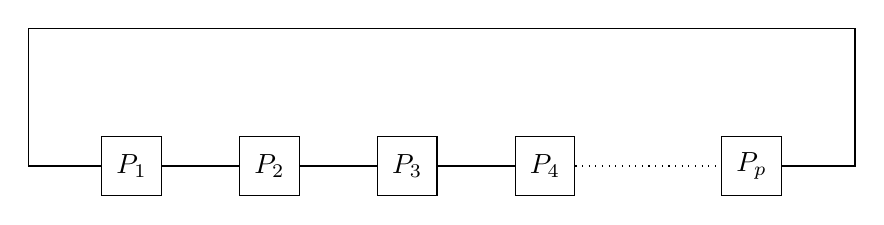
\begin{tikzpicture}
    [
        processor/.style={rectangle, draw, minimum size=5ex},
        scale=1.75,
    ]
    \node (p1) at (1,0) [processor] {$P_1$};
    \node (p2) at (2,0) [processor] {$P_2$};
    \node (p3) at (3,0) [processor] {$P_3$};
    \node (p4) at (4,0) [processor] {$P_4$};
    \node (pp) at (5.5,0) [processor] {$P_p$};
    \draw (p1) -- (p2) -- (p3) -- (p4);
    \draw [dotted] (p4) -- (pp);
    \draw (pp) -- (6.25,0) -- (6.25,1) -- (0.25,1) -- (0.25,0) -- (p1);
\end{tikzpicture}         

    \caption{Netzwerk in Form eines Rings}
    \label{ring}
\end{figure}

\begin{algorithm}
    \caption{Asynchronous Matrix Vector Product on a Ring \cite[S.18]{jaja}}
    \begin{algorithmic}[1]
    \Require (1) Nummer des Prozessors $i$; (2) Anzahl der Prozessoren $p$;
    (3) die $i$te Submatrix $B = A(1:n, (i-1)r+1:ir)$ der Größe $n \times r$ mit $r = \frac{n}{p}$;
    (4) der $i$te Subvektor $w = x((i-1)r+1:ir)$ der Länge $r$
    \Ensure Prozessor $P_i$ berechnet den Vektor $y = A_1x_1 + \cdots + A_ix_i$
    und gibt das Ergebnis nach rechts. Bei Terminierung hat $P_1$ das Ergebnis $Ax$.
    \State Berechne das Prudukt $z \gets Bw$
    \If {$i = 1$}
        \State $y \gets 0$
    \Else
        \State \textbf{receive}($y$, left)
    \EndIf
    \State $y \gets y + z$
    \State \textbf{send}($y$, right)
    \If {$i = 1$}
        \State \textbf{receive}($y$, left)
    \EndIf
    \end{algorithmic}
\end{algorithm}


\subsection{Parallel Random Access Machine}
Eine Parallel Random Access Machine, im folgenden PRAM, ist ein oft genutztes Maschinenmodell, um parallele Algorithmen zu analysieren.
Als eine Erweiterung der RAM, besteht sie aus $p$ Prozessoren, von denen jeder wiederum eine RAM ist, und einer globalen Speichereinheit (\emph{shared memory}).
Jeder Prozessor besitzt einen lokalen Speicher und führt ein lokales Programm aus.
Da sich die Instruktionen, die in einer Zeiteinheit ausgeführt werden, grundsätzlich unterscheiden können, gibt es sowohl MIMD als auch SIMD PRAM.
Die RAMs sind nicht direkt miteinander verbunden, verfügen jedoch über die Anweisungen \emph{global read(X,Y)} und \emph{global write(X,Y)}, mit denen Speicherblöcke aus bzw. in dem shared Memory kopiert werden können.
Der Umfang der Kommunikation zwischen den Prozessoren ist die Menge an Daten, welche zwischen den lokalen und dem globalen Speicher übermittelt wird.
Jedem Prozessor ist zusätzlich seine eigene Identität bekannt, so dass bedingte Anweisungen ermöglichen, Blöcke nur auf bestimmten Prozessoren auszuführen.
Die Operationenkomplexität einer PRAM ist das Produkt aus der Anzahl der verwendeten Prozessoren und der Zeitkomplexität.
\cite[S.9ff.]{jaja}


\subsubsection{Zugriffsbeschränkungen}
Für PRAM Modelle existieren verschiedene Beschränkungen in Bezug auf simultanen Zugriff auf den globalen Speicher.
Die verschiedenen Modelle sind unterschiedlich mächtig. Sie lassen sich unter erhöhtem Ressourcenverbrauch jedoch gegenseitig simulieren.
Im Folgenden sind die üblichen Variationen in aufsteigender Mächtigkeit aufgelistet.
Bei der EREW PRAM kann ein Prozessor zur Zeit eine Speicherzelle auslesen (\emph{exclusive read}) und schreiben (\emph{exclusive write}).
Die CREW lässt mehrere Prozessoren gleichzeitig aus der selben Speicherzelle lesen (\emph{concurrent read}), der Schreibzugriff ist jedoch auf einen Prozessor pro Zeiteinheit begrenzt.
Die CRCW PRAM erlaubt sowohl simultanen Lesezugriff als auch simultanen Schreibzugriff (\emph{concurrent write}).
Bei letzterem können Konflikte entstehen, wenn verschiedene Prozessoren versuchen, gleichzeitig in die selbe Speicherzelle zu schreiben. Diese werden durch verschiedene Subtypen behandelt werden.
Die \emph{common CRCW} lässt einen gleichzeitigen Schreibzugriff nur zu, falls alle beteiligten Prozessoren den gleichen Wert schreiben.
Beim \emph{arbitrary CRCW} schreibt ein beliebiger Prozessor in die Speicherzelle.
Die \emph{priority CRCW} gibt dem beteiligten Prozessor mit der höchsten Priorität (z.\,B. mit der niedrigsten ID) den Schreibzugriff.
Bei der Entwicklung von Algorithmen muss auf die Eigenschaften der verwendeten PRAM eingegangen werden. Beispielsweise darf es bei einem arbitrary CRCW keine Rolle spielen, welcher der Prozessoren in einem Schritt den Schreibzugriff bekommt.
\cite[S.14f.]{jaja}
